\documentclass{article} 
\usepackage[utf8]{inputenc}
\usepackage[T2A]{fontenc}
\usepackage[russian, english]{babel}
\usepackage{graphicx}	
\usepackage{amsmath, amssymb}
\usepackage{titlesec}
\newcommand\tab[1][1cm]{\hspace*{#1}}
\usepackage[14pt]{extsizes}
\usepackage{setspace,amsmath}
\usepackage[left=20mm, top=15mm, right=15mm, bottom=15mm, nohead, footskip=10mm]{geometry} 
\usepackage{mathtext}
\usepackage[dvipsnames]{xcolor}
\usepackage{ragged2e}
\usepackage{float}
\sloppy
\usepackage{caption}
\usepackage{hyperref}
%code highlighting
\usepackage{minted}

% colors
\definecolor{blue}{RGB}{17, 85, 204}
\definecolor{monokaibg}{HTML}{272822}

\hypersetup{
    colorlinks=true,
    linkcolor=black,
    urlcolor=blue
}

\graphicspath{ {img/} }
%--------------------------------------------------------------------
\begin{document}                                                         
\newpage
\thispagestyle{empty}

\begin{center}
Федеральное государственное образовательное бюджетное учреждение\\ высшего профессионального образования\\ 
\textbf{«Финансовый университет при Правительстве Российской Федерации»}\\
\end{center}
	
\vspace{2em}
	
\begin{center}
\textbf{Департамент анализа данных, принятия решения и финансовых технологий}\\ 
\end{center}
	
\vspace{2em}
	
\begin{center}
\textbf{Курсовая работа\\
\vspace{3mm}}
по дисциплине \textbf{"Технологии анализа данных и машинное обучение"} на тему: \\ \vspace{2em} \textbf{"Разработка подходов и алгоритмов для сбора и разметки лингвистических и семантических наборов данных большого объема"}\\
\vspace{3mm}
Вид исследуемых данных: Банковские транзакции\\
\end{center}
	
\vspace{6em}
		
\begin{flushright}
Выполнил:\\
студент группы ПМ17-2\\
Бахматов А. В.\\
Научный руководитель:\\
доцент\\
Макрушин Сергей Вячеславович
\end{flushright}

\vspace{\fill}
	
\begin{center}
Москва 2020
\end{center}

%--------------------------------------------------------------------
\newpage
	
\renewcommand*\contentsname{Содержание}
\makeatletter
\renewcommand{\l@section}{\@dottedtocline{1}{0em}{2em}}
\renewcommand{\l@subsection}{\@dottedtocline{1}{0em}{2.6em}}
\renewcommand{\l@subsubsection}{\@dottedtocline{1}{0em}{3.2em}}

\makeatother
\setcounter{page}{2}

\begin{center}
	\tableofcontents
\end{center}
%--------------------------------------------------------------------
\newpage
\addcontentsline{toc}{section}{Введение}
\section*{Введение}
\tab В данный момент технологии позволяют записывать и хранить массивные объемы данных о самых разных аспектах мира. Еженедельный приток информации на отдельных сайтах числится в терабайтах. Один из основных способов их структуризации и анализа - разметка, то есть разделение на категории. Размечать данные может либо человек, либо созданная для этой цели модель. Особенность больших данных состоит в том, что они по определению слишком массивны для того, чтобы процессом разметки полностью занимались люди. Поэтому вручную пытаться анализировать эту информацию просто невозможно, и необходимо для этого использовать модели машинного обучения. \\
\tabВ настоящее время машинное обучение стало флагманом IT-индустрии, о нем наслышаны все, его внедряют в самых разных сферах общества. Исключением не стала и банковская сфера: банки располагают большим количеством информации о своей деятельности и желают использовать ее для корректировок своей политики, принятия прибыльных решений.\\
\tabЦелью данной работы является классификация записей банковских транзакций (данные Газпромбанка) по текстовым данным и дополнительным признакам, используя модели машинного обучения. Достижение этой цели позволит банку автоматически группировать транзакции в группы, проводить над ними детальный анализ для дальнейшего принятия решений в управлении банком.\\
\tabРабота будет реализована на языке программирования Python 3.7 и будет состоять из попытки разметки данных с учителем (то есть на основе небольшой размеченной выборки) при помощи нескольких моделей: метода опорных векторов и искусственных сверточных нейронных сетей.\\
%--------------------------------------------------------------------
\newpage
\section{Теоретическая часть} 
%--------------------------------------------------------------------
\subsection{Задачи обработки естественного языка и ее проблематика}
\tab Natural language processing (NLP) - это набор подходов компьютерной обработки естественных языков. Его основные задачи:\\
\tab\tab1) Классификация текста: отнесение текста к одному из заранее определенных классов. Примеры: фильтр спама, анализ тональности, определение темы текста;\\
\tab\tab2) Кластеризация текста: деление текстов на группы (кластеры). Примеры: агрегация новостей, рекомендательные системы;\\ 
\tab\tab3) Машинный перевод;\\ 
\tab\tab4) Текстовый анализ. Примеры: распознавание именованных сущностей (при имеющемся наборе сущностей, отнести каждое слово к одному из них), нахождение семантических связей между словами;\\ 
\tab\tab5) Распознавание речи;\\
\tab\tab6) Проверка правописания;\\
\tab\tab7) Генерация текста.\\
\\
\tabОсновные проблемы, возникающие при обработке языка:\\
\tab\tab1) Контекст слов: у слов зачастую имеется несколько значений, которые зависят от контекста слова в предложении, а так же от времени, в которое текст был написан, и от интенции пишущего (сарказм);\\
\tab\tab2) Опечатки, мусор в тексте (например, в html), множество форм у одного слова.\\
%--------------------------------------------------------------------
\subsection{Этапы обработки текста} 
\tabПри создании алгоритмов обработки текста обычно используют следующие процедуры:\\
\tab\tab1) Токенизация: разбиение текста на составные части - токены (обычно слова, но в некоторых задачах имеет смысл выделять знаки препинания как отдельные токены, например, при обработке текста с форумов и социальных сетей);\\
\tab\tab2) Очистка незначащих слов (стоп-слов);\\
\tab\tab3) Лемматизация: приведение слов к их леммам - начальным формам;\\
\tab\tab4) Стемминг: приведение слов к их основам. Более простой аналог лемматизации (как пример: при лемматизации слово "сделали" будет преобразовано в "сделать", а при стемминге - в "сделал");\\
\tab\tab5) Исправление опечаток;\\
\tab\tab6) Представление текста (encoding) - перевод текста в более простую для обработки форму. Популярные виды представления текста:\\
\tab\tab\tab а) мешок слов - каждое предложение выражается как вектор, показывающий, сколько раз каждое слово из корпуса встречается в предложении (т.е. показывается, какие слова находятся в данном предложении, а какие нет);\\ 
\tab\tab\tab б) TF-IDF - похож на мешок слов, но вместо количества у каждого слова, которое есть в конкретном предложении, имеется величина, расчитываемая как TF*IDF, где TF (Term Frequency) - частота встречаемости слова в предложении, а IDF (Inverse Document Frequency) - обратная частота встречаемости слова во всем корпусе. Величина IDF позволяет игнорировать слова, которые встречаются очень часто, а следовательно, не несут информации. Таким образом, величина TF-IDF вычисляет "полезность слова";\\
\tab\tab\tab в) представление метками (Label Encoding) - каждый токен представляется уникальной числом;\\
\tab\tab\tab г) представление унитарным кодом (One-hot Encoding) - аналог Label Encoding, но вместо числа - вектор-индикатор;\\
\tab\tab\tab д) векторное представление токенов (ембеддинги): каждый токен представляется как n-мерный вектор, чье значение отображает его связи с остальными токенами в корпусе (т.е. чем ближе векторы разных токенов, тем они более похожи по смыслу).\\ 
\tab Среди различных видов представлений текста, мешок слов и TF-IDF не сохраняют порядок слов в предложении и смысла слов, но при этом довольно просто реализуются. Эмбеддинги имеют более сложную реализацию, но сохраняют порядок слов, и каждое слово имеет относительный смысл.\\
%--------------------------------------------------------------------
\subsection{Модели классификации}
\tab Для классификации текста используется множество моделей:\\
\tab\tab1) Наивный байесовский классификатор - один из самых простых классификаторов, который для предсказания классов считает частоты слов и классов в корпусе. Считает вероятность появления каждого слова независимым от других;\\
\tab\tab2) Логистическая регрессия: простой вид искусственной нейронной сети, имеющей лишь входной и выходной слои;\\
\tab\tab3) Метод опорных векторов: разделяет пространство векторов гиперплоскостью. Метод может работать на уровне нейронных сетей со сложной архитектурой, и при этом не имеет большого количество параметров;\\
\tab\tab4) Нейронные сети прямого распространения: принцип работы тот же, что и у логистической регрессии, но имеет скрытые слои;\\
\tab\tab5) Сверточные нейронные сети: обычно используются для работы с фото, но полезны также для текста (ибо при представлении текста ембеддингами на входе имеем двухмерную матрицу);\\
\tab\tab6) Рекуррентные нейронные сети: главная особенность - передача данных между узлами на одном и том же слое, из-за чего возможно сохранять контекст. Из-за этого требуют больше ресурсов для обучения.\\
\tabМы для классификации будем использовать 1-мерную сверточную нейронную сеть.\\
%--------------------------------------------------------------------
\section{Построение моделей} 
\subsection{Постановка задачи и датасет}
\tab Датасет имеет следующие признаки: documentid, to\_acc, name\_to, from\_acc, name\_from, purp, sum, payer\_tax\_num, payee\_tax\_num, payer\_bank\_bic\_cd, payee\_bank\_bic\_cd, inn\_same, bic\_same, class, payer\_ОКВЭД\_main, payee\_ОКВЭД\_main. Из интересующих нас признаков имеются  purp - текстовое описание транзакции (например "За электроснабжение (окончательный расчет, за январь), по договору N КП-13-Н/309 от 01.01.2018. С/ф N 3010119120000385/12/00000 от 31.01.2019Сумма 98898-65В т.ч. НДС 20\% 16483-11"), to\_acc и from\_acc - на какой и с какого счета производится транзакция, payer\_ОКВЭД\_main и payee\_ОКВЭД\_main - счета ОКВЭД (Общероссийский классификатор видов экономической деятельности).\\
\tab Транзакцию нам нужно отнести к одному из классов: Комиссии банку, Суды, Зарплата, Аренда, Валюта, Инкассирование, Эквайринг, Возврат, Штрафы прочие, Штрафы государство, Проценты по кредиту, Страховое возмещение, Налоги НДФЛ, Налоги прочие, Налоги прибыль, Налоги НДС, Депозит, Вексель, Кредит, Оплата ФЛ, Выручка, Пополнение счета, Перевод на ФЛ, Займ, Выплаты соцхарактера, Взыскание с ФЛ, Страховая премия, Обеспечение, Пожертвования и благотворительность, Дивиденды, Прочее.\\
\tab Датасет включает в себя 3300 размеченных строк (20000 всего).\\
%--------------------------------------------------------------------
\subsection{Сверточная нейронная сеть}
\subsubsection{Предобработка}
\tab Загрузим датасет и уберем строки в которых есть nan:\\
\begin{minted}
[
style=monokai,
bgcolor=monokaibg,
breaklines,
baselinestretch=1.2,
fontsize=\small
]{python}
def load_data(path):
  data = pd.read_csv(path)
  data.rename({'Ответ 2 из 3:':'class'}, axis=1, inplace=True)
  return data

train_path = get_drive_path('data\\train_data_3300_win.txt')
test_path = get_drive_path('data\\test_data_3300_win.txt')

train_data = load_data(train_path)
test_data = load_data(test_path)
all_data = pd.concat((train_data, test_data))
\end{minted} 
\begin{figure}[H]
\centering
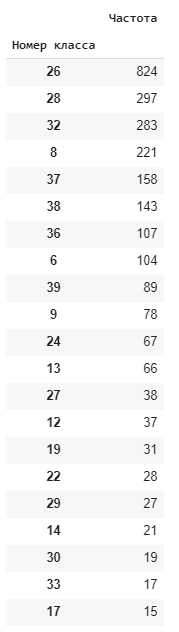
\includegraphics[width=4cm]{class_freq.png}
\caption{Частоты классов (названия представлены числами)}
\end{figure}
\tabПредобработка текста состоит из очистки от дат (get\_clear\_text), токенизации по словам, замены токенов из 20 цифр в "карта", очистки от чисел и нелексикографических символов\\
\begin{minted}
[
style=monokai,
bgcolor=monokaibg,
breaklines,
baselinestretch=1.2,
fontsize=\small
]{python}
def remove_noise(tokens, stop_words = []):
    
    cleaned_tokens = []
    
    for token in tokens:
        
        #номера карт (весь токен это 20 цифр)
        token = "карта" if re.search(r"^\d{20}$", token) else token
        #убираем числа
        token = re.sub(r'\d', '', token)
        #очистка нелексигографических символов
        token = re.sub(r'\W', '', token)
        
        #убираем токены состояющие из одного символа или являющиеся стоп-словом
        if len(token) > 1 and token.lower() not in stop_words:
            cleaned_tokens.append(token.lower())
                
    return cleaned_tokens

def get_cleaned_features(features, stop_words): 
    sentences_tokens = [word_tokenize(get_clear_text(sentence)) for sentence in features]
    return [remove_noise(tokens, stop_words) for tokens in sentences_tokens]
\end{minted}


\tabФункция для предобработки данных (очистки, разбиения на подвыборки, приведения слов к числам)\\

\begin{minted}
[
style=monokai,
bgcolor=monokaibg,
breaklines,
baselinestretch=1.2,
fontsize=\small
]{python}
def get_data_for_nn(data, no_other_features=False, max_len=None, all_data=None, test=False, tokenizer=None, encoder_dict=None, y_encoder=None, path_to_shortenings_file=None, fix_spelling=False):
  
  stop_words = stopwords.words('russian')

  X, y = data['purp'], data['class']
  X_text = X
  #чистка текста
  X = get_cleaned_features(X, stop_words, path_to_shortenings_file, fix_spelling)
  
  if not test and not no_other_features:
    y, y_encoder = encode(y, OneHotEncoder, all_data['class'])
    other_features, encoder_dict = extract_features(data)
    other_features, X, y = dropna(other_features, X, y)
    #валидационная выборка
    X, X_val, y, y_val, other_features, other_features_val, X_text, X_text_val = train_test_split(X, y, other_features, X_text, test_size=0.2, stratify=y, random_state=42)
    #слова в числа
    tokenizer = Tokenizer(num_words=10000)
    tokenizer.fit_on_texts(X)
    X = tokenizer.texts_to_sequences(X)
    X_val = tokenizer.texts_to_sequences(X_val)
    max_len = len(max(X, key=len)) 
    #паддинг
    X = pad_sequences(X, padding='post', maxlen=max_len)
    X_val = pad_sequences(X_val, padding='post', maxlen=max_len)

    return X, X_val, y, y_val, X_text, X_text_val, other_features, other_features_val, tokenizer, encoder_dict, y_encoder
  
  elif not test:
    y, y_encoder = encode(y, OneHotEncoder, all_data['class'])
    #валидационная выборка
    X, X_val, y, y_val, X_text, X_text_val = train_test_split(X, y, X_text, test_size=0.2, stratify=y, random_state=42)
    #слова в числа
    tokenizer = Tokenizer(num_words=10000)
    tokenizer.fit_on_texts(X)
    X = tokenizer.texts_to_sequences(X)
    X_val = tokenizer.texts_to_sequences(X_val)
    max_len = len(max(X, key=len)) 
    #паддинг
    X = pad_sequences(X, padding='post', maxlen=max_len)
    X_val = pad_sequences(X_val, padding='post', maxlen=max_len)

    return X, X_val, y, y_val, X_text, X_text_val, tokenizer, y_encoder

  elif test and not no_other_features:
    y = encode(y, y_encoder)
    other_features = extract_features(data, encoder_dict) 
    
    #слова в числа
    X = tokenizer.texts_to_sequences(X)
    #паддинг
    X = pad_sequences(X, padding='post', maxlen=max_len)
    
    return X, y, other_features, X_text

  else:
    y = encode(y, y_encoder) 
    #слова в числа
    X = tokenizer.texts_to_sequences(X)
    #паддинг
    X = pad_sequences(X, padding='post', maxlen=max_len)
   
    return X, y, X_text
\end{minted}

\tab Функция для загрузки ембеддингов с помощью предобученной модели fasttext\\

\begin{minted}
[
style=monokai,
bgcolor=monokaibg,
breaklines,
baselinestretch=1.2,
fontsize=\small
]{python}
def load_fast_text_pretrained_oov(corpus, output_file_path, path_to_model, tokenizer, number_of_dimensions):
    """
    Загрузить embedding_matrix из предобученных векторов fasttext
    """
    try:
        embedding_matrix = load_embedding(output_file_path, tokenizer)
    except FileNotFoundError:
        ft_model = FastTextKeyedVectors.load(path_to_model)
        model_to_vec_file(corpus, output_file_path, ft_model.__getitem__, number_of_dimensions)
        embedding_matrix = model_to_matrix(ft_model.__getitem__, tokenizer, number_of_dimensions)
    
    return embedding_matrix
\end{minted}

\tabСоздадим тренировочную и валидационную выборку, сформируем дополнительные признаки как one-hot матрицу нграмм, загрузим предобученную fasttext модель out-of-vocabulary\\

\begin{minted}
[
style=monokai,
bgcolor=monokaibg,
breaklines,
baselinestretch=1.2,
fontsize=\small
]{python}
X_train, X_val, y_train, y_val, X_text_train, X_text_val, tokenizer, y_encoder = get_data_for_nn(train_data, no_other_features=True, all_data=all_data)
cleaned_train_data = train_data[['purp','class']].copy().rename({'class':'class_number'}, axis=1)

cleaned_train_data['purp'] = [' '.join(sentence) for sentence in get_cleaned_features(train_data['purp'], stop_words)]
ngrams = utils.NGramsCounter(cleaned_train_data).choose_significant_ngrams(2, 9, 0.7).columns
other_features_train = np.array([[int(ngram in ' '.join(sentence)) for ngram in ngrams] for sentence in get_cleaned_features(X_text_train, stop_words)])
other_features_val = np.array([[int(ngram in ' '.join(sentence)) for ngram in ngrams] for sentence in get_cleaned_features(X_text_val, stop_words)])

vocab_size = len(tokenizer.word_index)+1
max_len = X_train.shape[1]
output_number = y_train.shape[1]

path_to_model = get_drive_path("data\\fasttext\\geowac_tokens_none_fasttextskipgram_300\\model.model")
output_file_path = get_drive_path(f"data\\fasttext\\ft_geowac_oov_300_{cleaned_corpus_version}.vec")

embedding_matrix = eb.load_fast_text_pretrained_oov(cleaned_corpus, output_file_path, path_to_model, tokenizer, number_of_dimensions)
\end{minted}
\subsubsection{Построение и обучение модели}
\tab Построение и обучение будет реализовано при помощи библиотеки keras.\\
\tabОпределим функции f1 micro и f1 weighted для оценки качества модели\\
\begin{minted}
[
style=monokai,
bgcolor=monokaibg,
breaklines,
baselinestretch=1.2,
fontsize=\small
]{python}
import keras.backend as K
from sklearn.metrics import f1_score

def f1(true, pred, average='micro', loss=False): #shapes (batch, output_number) 
    if not loss:
        predLabels = K.argmax(pred, axis=-1)
        pred = K.one_hot(predLabels, output_number) 

    ground_positives = K.sum(true, axis=0)       # = TP + FN
    pred_positives = K.sum(pred, axis=0)         # = TP + FP
    true_positives = K.sum(true * pred, axis=0)  # = TP
    
    if average == 'micro':
        true_positives = K.sum(true_positives)
        pred_positives = K.sum(pred_positives)
        ground_positives = K.sum(ground_positives)
    
    precision = (true_positives + K.epsilon()) / (pred_positives + K.epsilon()) 
    recall = (true_positives + K.epsilon()) / (ground_positives + K.epsilon()) 
        #both = 1 if ground_positives == 0 or pred_positives == 0
        #shape (output_number,)

    f1 = 2 * (precision * recall) / (precision + recall + K.epsilon())
        #not sure if this last epsilon is necessary
        #mathematically not, but maybe to avoid computational instability
        #still with shape (output_number,)
    
    if average == 'weighted':
        f1 = f1 * ground_positives / K.sum(ground_positives)
        f1 = K.sum(f1)
    
    return f1 if not loss else 1-f1

def f1_micro(true, pred):
    return f1(true, pred, average='micro', loss=False)
    
def f1_weighted(true, pred):
    return f1(true, pred, average='weighted', loss=False)
\end{minted}
\tabПостроим модель (текстовые данные в виде числовых последовательностей поступают преобразуются в ембеддинги, последовательность ембеддингов поступает в сверточный слой, потом проходит через слои макс пулинга, соединяется с дополнительными признаками и получившийся слой соединяется с выходным)\\
\begin{minted}
[
style=monokai,
bgcolor=monokaibg,
breaklines,
baselinestretch=1.2,
fontsize=\small
]{python}
from keras.layers import Input, Concatenate, Flatten, Dense
from keras.models import Model

loss = 'categorical_crossentropy'
activation = 'softmax'
filters, kernel_size = 10, 5

text_input = Input(shape=(max_len,))
vector_input = Input(shape=(other_features_train.shape[1],))

embedding_layer = Embedding(input_dim=vocab_size, 
                            output_dim=number_of_dimensions,
                            weights=[embedding_matrix], 
                            input_length=max_len, 
                            trainable=True,
                            embeddings_regularizer=reg.l1(0.0005))(text_input)
conv_layer = Conv1D(filters, kernel_size, activation='relu', kernel_regularizer=reg.l2(0.005))(embedding_layer)
conv_layer = Dropout(0.2)(conv_layer)
conv_layer = MaxPooling1D(10)(conv_layer)
conv_layer = GlobalMaxPooling1D()(conv_layer)

concat_layer = Concatenate()([vector_input, conv_layer])
output = Dense(output_number, activation=activation)(concat_layer)

model = Model(inputs=[text_input, vector_input], outputs=output)
model.compile(optimizer=Adam(learning_rate=0.01), loss=loss, metrics=['acc',f1_micro,f1_weighted])
model.summary()
\end{minted}
\begin{figure}[H]
\centering
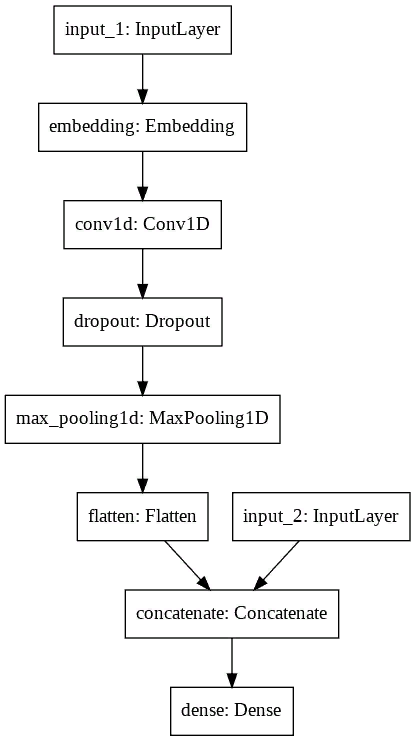
\includegraphics[width=17cm]{conv other features arch.png}
\caption{Одномерная сверточная нейронная сеть с двумя входными слоями}
\end{figure}
\tabОбучим модель.\\
\begin{minted}
[
style=monokai,
bgcolor=monokaibg,
breaklines,
baselinestretch=1.2,
fontsize=\small
]{python}
filepath = get_drive_path("saved models\\saved-model-conv.hdf5")
checkpoint = ModelCheckpoint(filepath, monitor='val_f1_micro', verbose=0, save_best_only=True, mode='max', save_weights_only=True)
early_stop = EarlyStopping(monitor='val_f1_micro', mode='max', verbose=1, patience=20)

callbacks = [checkpoint, early_stop]
batch_size = 128
epochs = 50

history = model.fit([X_train,other_features_train],
                    y_train,
                    batch_size=batch_size, 
                    epochs=epochs,
                    callbacks=callbacks,
                    validation_data=([X_val,other_features_val], y_val)
                   )
\end{minted}
\begin{figure}[H]
\centering
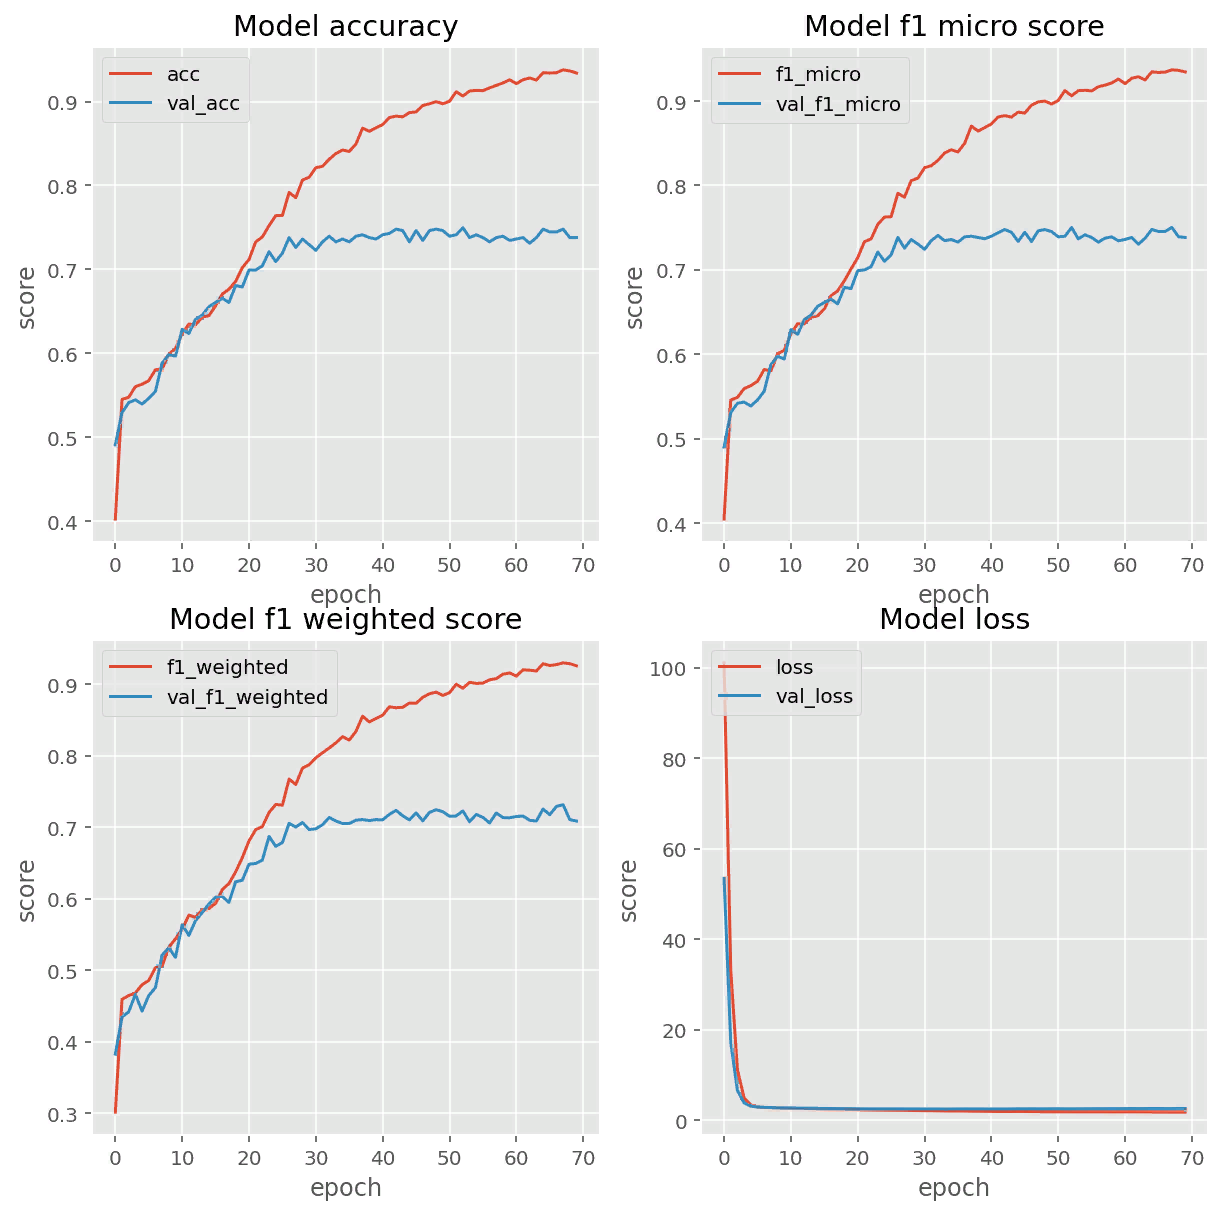
\includegraphics[width=16cm]{evaluation.png}
\caption{Оценка модели на эпохах обучения}
\end{figure}

\subsection{Метод опорных векторов}

\subsubsection{Предобработка, построение и обучение модели}

\tab На вход методу опорных векторов будет подаваться связка TF-IDF и one-hot нграмм, коррелирующих с классами на 0.7 или более.\\
\tab Почистим данные теми же методами, что и ранее, и сформируем one-hot матрицу.\\

\begin{minted}
[
style=monokai,
bgcolor=monokaibg,
breaklines,
baselinestretch=1.2,
fontsize=\small
]{python}

cleaned_train_data = train_data[['purp',target_name]].copy()
stop_words = stopwords.words('russian')

cleaned_train_data['purp'] = [' '.join(sentence) for sentence in get_cleaned_features(train_data['purp'], stop_words)]
train_ngrams = utils.NGramsCounter(cleaned_train_data).choose_significant_ngrams(2, 9, 0.7)

cleaned_test_data = test_data[['purp',target_name]].copy()
cleaned_test_data['purp'] = [' '.join(sentence) for sentence in get_cleaned_features(test_data['purp'], stop_words)]
test_ngrams = np.array([[int(ngram in sentence) for ngram in train_ngrams.columns] for sentence in cleaned_test_data['purp']])
\end{minted}

\tab Сформируем TF-IDF матрицу, склеим ее с one-hot матрицей, и обучим SVM линейным ядром.\\

\begin{minted}
[
style=monokai,
bgcolor=monokaibg,
breaklines,
baselinestretch=1.2,
fontsize=\small
]{python}
vectorizer = TfidfVectorizer()
train_vectors = vectorizer.fit_transform(train_data['purp'])
train_vectors = np.hstack((train_vectors.toarray(),train_ngrams))
test_vectors = vectorizer.transform(test_data['purp'])
test_vectors = np.hstack((test_vectors.toarray(),test_ngrams))

classifier_svm = LinearSVC()
classifier_svm.fit(train_vectors, train_data[target_name])
\end{minted}

\section{Оценка моделей}
\subsection{Выбор метрики}

\tab Для моделей классификации существует множество метрик для оценки качества прогнозов, самая простая - это точность, однако она может быть обманчива (чаще всего это происходит в датасетах с несбалансированным количеством классов). Метрики, использующиеся для вычисления большинства остальных, это precision и recall, которые показывают ошибки первого и второго рода (false negatives and false positives), считаются они по формулам true positivies / (true positivies + false positivies) и true positivies / (true positivies + false negatives) соответственно. В нашей задаче нельзя выделить, что важнее: не совершить ошибку первого или второго рода, поэтому логично использовать усредненную величину. В качестве такой величины мы будем использовать F1, являющейся сглаженной средней между precision и recall (2 * (precision * recall) / (precision + recall)). Стоит отметить, что эти метрики изначально расчитывают ошибки в бинарной классификации, а для обобщения на классификацию произвольного числа классов используется чаще всего метод один-против-остальных (one-vs-rest): один класс рассматривается как положительный, и все остальные - как отрицательный. Таким образом, у каждого класса будет свой набор recall, precision и f1. Для нахождения среднего f1 мы будем использовать два метода: взвешенный и микро. Взвешенный метод берет среднее взвешеннее значение всех f1 (весами является количество представителей класса в датасете). Микро глобально считает общее число true positives, false negatives, false positives и на их основе считает f1.

\subsection{Оценка моделей на тестовой выборке}

\tabДля оценки нейронной сети выберем ту, у которой наибольшая валидационная f1 micro.\\

\begin{minted}
[
style=monokai,
bgcolor=monokaibg,
breaklines,
baselinestretch=1.2,
fontsize=\small
]{python}
conv1d_model_other_features.load_weights(get_drive_path('saved models\\saved-model-conv-other-features.hdf5'))

X_test, y_test, X_text_test = get_data_for_nn(test_data, no_other_features=True, all_data=all_data, test=True, tokenizer=tokenizer, y_encoder=y_encoder)
other_features_test = np.array([[int(ngram in ' '.join(sentence)) for ngram in ngrams] for sentence in get_cleaned_features(X_text_test, stop_words)])

pred = np.round(conv1d_model_other_features.predict([X_test, other_features_test]))

print('f1 micro', np.round(f1_score(y_test, pred, average='micro'), 4))
print('f1 weighted', np.round(f1_score(y_test, pred, average='weighted'), 4))
\end{minted}
\tabПолучаем f1 micro 0.7672, f1 weighted 0.7296.\\
 
\tabОценка метода опорных векторов:\\

\begin{minted}
[
style=monokai,
bgcolor=monokaibg,
breaklines,
baselinestretch=1.2,
fontsize=\small
]{python}
prediction = classifier_svm.predict(test_vectors)

print('f1 micro:', f1_score(test_data[target_name], prediction, average='micro'))
print('f1 weighted:', f1_score(test_data[target_name], prediction, average='weighted'))
\end{minted}

\tab f1 micro 0.8217, f1 weighted 0.8098.\\

\newpage
\addcontentsline{toc}{section}{Заключение}
\section*{Заключение}

\tab Для задачи разметки лингвистических данных большого объема было выбрано использовать подходы NLP и машинного обучения: на размеченной выборке малого размера обучаются модели. Была проведена чистка текстовых данных, перебор разных конфигураций:\\
\tab\tab ембеддингов: word2vec, fasttext, которые были либо обучены на датасете, либо предобучены;\\
\tab\tab дополнительных признаков: из столбцов датасета или по нграммам;\\
\tab\tab архитектур нейронной сети и их гиперпараметров.\\
\tab В итоге на тестовой выборке лучше всего себя показал метод опорных векторов. Несмотря на полезность нейронных сетей из-за их гибкости, эта самая гибкость требует большой настройки, которая не всегда приводит к положительным результатам.

\newpage
\addcontentsline{toc}{section}{Список использованных источников}
\section*{Список использованных источников}
\renewcommand{\refname}{}
\begin{thebibliography}{7}
\bibitem{i1} Applied Text Analysis with Python by Benjamin Bengfort, Rebecca Bilbro, and Tony Ojeda (O’Reilly). 978­1­491­96304­3
\bibitem{i2} Автоматическая обработка текстов на естественном языке и анализ данных : учеб. пособие / Большакова Е.И., Воронцов К.В., Ефремова Н.Э., Клышинский Э.С., Лукашевич Н.В., Сапин А.С. — М.: Изд-во НИУ ВШЭ, 2017. — 269 с. ISBN 978–5–9909752-1-7
\bibitem{i3}МЕТОДЫ И МОДЕЛИ АВТОМАТИЧЕСКОГО ИЗВЛЕЧЕНИЯ КЛЮЧЕВЫХ СЛОВ С.О. Шереметьева, П.Г. Осминин Вестник ЮУрГУ. Серия «Лингвистика». 2015. Т. 12, No 1. С. 76–81
\bibitem{i4}https://countwordsfree.com/stopwords/russian
\bibitem{i5}Automated News Categorization using Machine Learning
methods
U Suleymanov1
 and S Rustamov2,3
 Applying Machine Learning Algorithms for News Articles Categorization: Using SVM and kNN with TF-IDF Approach
 A Comparative Analysis Of News Categorization
Using Machine Learning Approaches
Nabamita Deb, Vishesh Jha, Alok K Panjiyar, Roshan Kr Gupta
\end{thebibliography}

\end{document}  